% !TeX encoding = UTF-8
% !TeX spellcheck = it_IT
% !TeX root = MatDiz.tex
\chapter{C} 
\vspace{5mm} 
\lemma{c} \titolettoa{simbolo} del grado centesimale.\titolettoa{simbolo} del capitale in matematica finanziaria.\titolettoa{simbolo} del cento nella numerazione latina.
\lemma{calcolo} Insieme di procedimenti atti a dare la soluzione di un dato problema matematico.\llemma{c. combinatorio}Parte della matematica che ha per scopo di contare i raggruppamenti di oggetti\pointsto~\vedilemma{permutazione}.
\lemma{campo}
\lemma{Cantor Georg} (1845 – 1918)\index{Cantor Georg}Fondatore della teoria degli insiemi introdusse il concetto di numero transfinito. 
\begin{figure}
	\centering
	\scaptionb{Georg Cantor (1845 – 1918)}
	\label{fig:georgcantor2}
	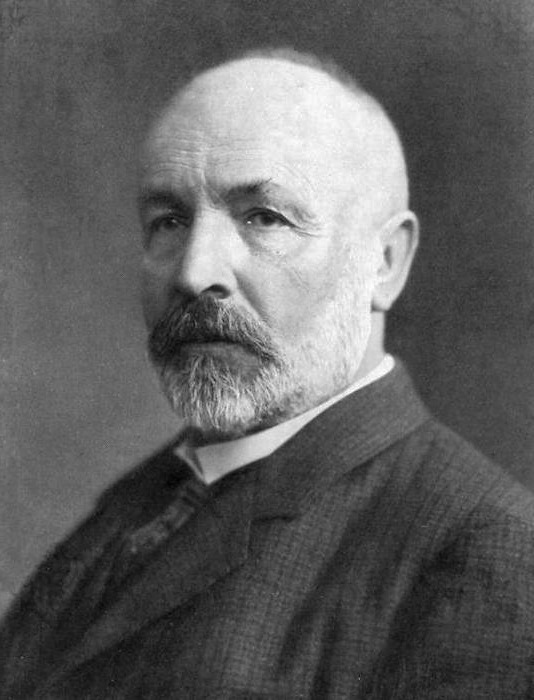
\includegraphics[width=0.7\linewidth]{Figure/C/Georg_Cantor2}
\end{figure}
\lemma{Cardano Gerolamo}(1501-1576)\index{Cardano Gerolamo}
\lemma{Cavalieri Bonaventura}(1598 1647)
\begin{figure}
	\centering
	\includegraphics[width=0.7\linewidth]{Figure/C/Jerôme_Cardan}
	\scaptionb{Girolamo Cardano (1501-1576)}
	\label{fig:jeromecardan}
\end{figure}
\begin{figure}
	\centering
	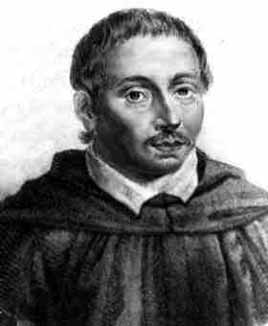
\includegraphics[width=0.7\linewidth]{Figure/C/Bonaventura_Cavalieri}
	\scaptionb{Cardano Gerolamo (1501-1576)}
	\label{fig:bonaventuracavalieri}
\end{figure}
\lemma{cateto} Lato di triangolo rettangolo\pointsto~\vedilemma{t. rettangolo} non opposto all'angolo retto\pointsto~\vedilemma{a. retto}.
\lemma{centro} Punto equidistante da tutti i punti della circonferenza.\llemma{c. delle masse} \pointsto~\vedilemma{baricentro} \cite{UTET1969} 
\llemma{c. di gravità} \'{E} il punto nel quale si può pensare applicata la forza peso del corpo.
\lemma{cicloide} Linea piana generata dal moto di un punto connesso rigidamente ad un cerchio che rotola senza strisciare.
\lemma{Chester Roberto di} \index{Chester Roberto di} Traduttore e arabista inglese lavorò intono al 1150. A lui si deve la prima traduzione parziale de libro \textit{al-Kitāb al-mukhtasar fī hisāb al-jabr wa al-muqābala} di al-Khwarizmi\pointsto~\vedilemma{al-Khwarizmi Muhammad ibn Musa} che tradusse in latino come \textit{Liber algebrae et almucabala} \cite{Gheverghese2000} 
\lemma{circonferenza} Luogo geometrico\pointsto~\vedilemma{luogo geometrico} dei punti del piano equidistanti da un punto fisso detto centro.\llemma{c. goniometrica} In un sistema di riferimento cartesiano\pointsto~\vedilemma{s. di riferimento cartesiano} è una circonferenza con centro nell'origine degli assi e raggio\pointsto~\vedilemma{raggio} unitario.\llemma{c. lunghezza} La lunghezza di una circonferenza di raggio $r$ è $l=2\pi r$.
\llemma{c. iscritta} 
\lemma{corda} Segmento\pointsto~\vedilemma{segmento} che congiunge due punti di una circonferenza\pointsto~\vedilemma{circonferenza} .
\lemma{coseno} Dato un triangolo rettangolo\pointsto~\vedilemma{t. rettangolo} definiamo coseno dell'angolo il rapporto tra il cateto\pointsto~\vedilemma{cateto} adiacente\pointsto~\vedilemma{s. adiacente} all'angolo e l'ipotenusa\pointsto~\vedilemma{ipotenusa} $\cos\beta=\frac{\text{adiacente} } {\text{ipotenusa} } $. Data una circonferenza goniometrica\pointsto~\vedilemma{c. goniometrica} diremo coseno l'ascissa\pointsto~\vedilemma{ascissa} del punto di intersezione tra il raggio\pointsto~\vedilemma{raggio} e la circonferenza \vref*{fig:cdefinizioneCoseno}.\llemma{c. funzione} 
\begin{figure} [b!]
	\scaptionb{Funzione coseno grafico} 
	\label{fig:cfunzioneCoseno} 
	\includestandalone[width=\linewidth]{Figure/cosenografico} 
\end{figure} 
La funzione coseno\pointsto~\vedilemma{goniometria} è definita in $\R$ a valore in $[-1,1]$. La funzione è limitata\pointsto~\vedilemma{f. limitata}.
La funzione è periodica\pointsto~\seeentry{f. periodica} di periodo $k\pi\quad k\in\Z$. La figura~\vref{fig:cfunzioneCoseno} rappresenta il grafico della funzione.
\lemma{coppia} Elemento dell'insieme prodotto cartesiano\pointsto~\vedilemma{p. cartesiano} $A\times B$. Si indica con $\left(a,b\right)\quad a\in A,\, b\in B$.\llemma{c. ordinata} Una coppia è ordinata se $\left(a,b\right)\neq\left(b,a\right)$. 
\lemma{crescente} \pointsto~\vedilemma{f. crescente} .
\begin{figure} 
	\scaptionb{Coseno definizione} 
	\label{fig:cdefinizioneCoseno} 
	\includestandalone[width=\linewidth]{Figure/cosenodefinizione} 
\end{figure} 